\section{Continuous Integration}

CI er en practice hvor udviklere integrere deres arbejde ofte. Ifølge Martin Fowler, gerne minimumn en gang dagligt. Hver integration verificeres med et automatisk build og test. På denne måde findes integrationsfejl tidligt.

\begin{figure}[H]
\centering
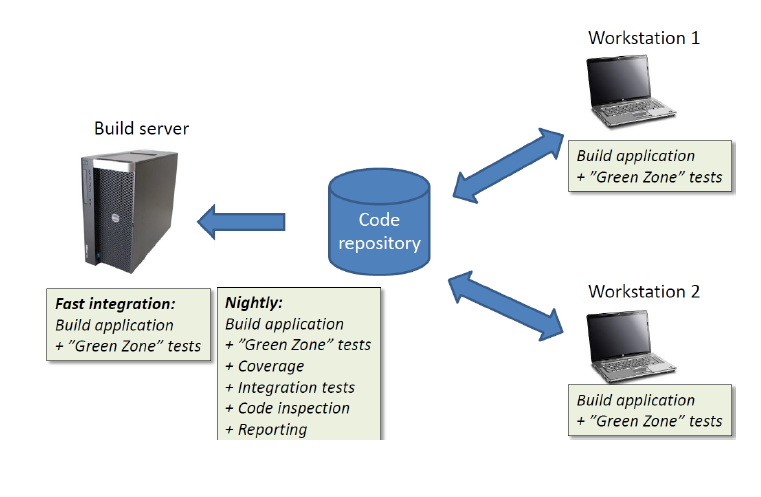
\includegraphics[width=0.7\linewidth]{figs/ciArch.PNG}
\caption{Modellen for Continous Integration i et projekt}
\label{fig:ciArch}
\end{figure}

\begin{figure}[H]
\centering
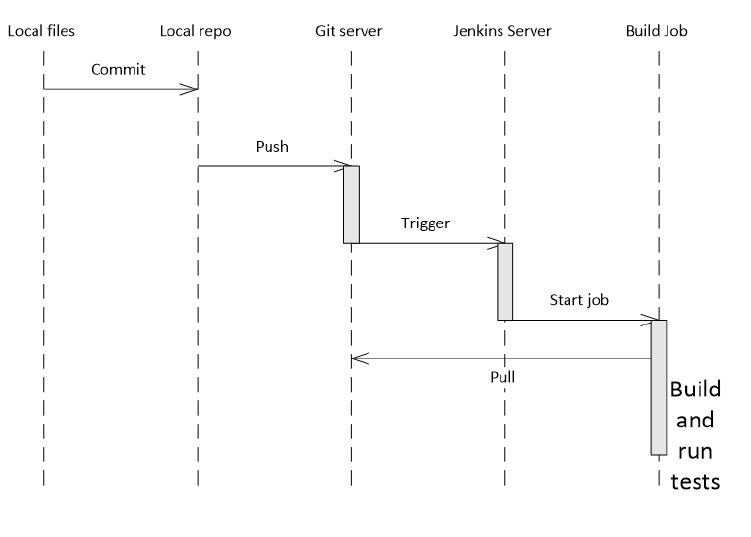
\includegraphics[width=0.8\linewidth]{figs/ciTriggerSeq.PNG}
\caption{Trigger sekvens for Continous Integration med Git repository.}
\label{fig:ciTriggerSeq}
\end{figure}

\subsection{CI funktionalitet}
På figur~\ref{fig:ciTriggerSeq} ses trigger sekvensen for et automatisk \textit{\textbf{build}} og \textit{\textbf{run}}. Nogle af fordelene ved Continous Integration er:

\begin{itemize}
	\item Hele systemet testes samlet.
	\item Test sker udenfor arbejds-miljøet - Ved store projekter spares tid.
	\item Løbende integration (skal ikke gøres alt sammen til sidst).
	\item Der pushes deployable builds.
	\item Vi kan få tests udført om natten.
	\item Der kan pushes ofte, så fejl findes tidligt før, ændringen bliver fór stor.
	\item Code metrics/quality er altid opdateret (hvis CI systemet understøtter det).
\end{itemize}

\subsection{Jenkins}
I SWT arbejdes der med Jenkins serveren. Udover at bygge et software projekt, kører den også tilhørende tests, hvorefter den kan sende en mail om resultatet.\\

Derudover er der meget funktionalitet i Jenkins. Herunder Code Coverage og Metrics, som er brugt i ATM opgaven. I denne opgave er Jenkins brugt til at køre tre forskellige opgaver, i nævnt rækkefølge som en \textit{pipeline}: 

\begin{enumerate}
	\item Unittests.
	\item Integrationstest.
	\item Metrics.
\end{enumerate}
